\documentclass{standalone}
\usepackage[utf8]{inputenc}
\usepackage[margin=25mm]{geometry}
\usepackage{tikz}
\usetikzlibrary{shapes.multipart}
\begin{document}
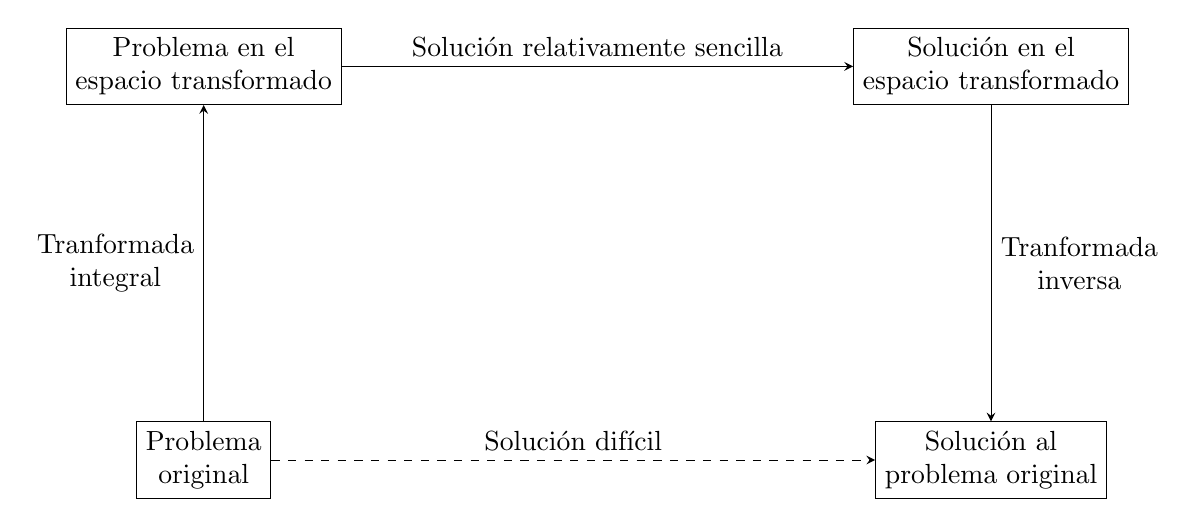
\begin{tikzpicture}[every text node part/.style={align=center}, >=stealth, node distance = 5cm, auto]
	\node (cuadro1) [rectangle, draw] {Problema \\ original};
	\node (cuadro2) [above of = cuadro1, rectangle, draw] {Problema en el \\ espacio transformado};
	\node (cuadro3) [right of = cuadro2, rectangle, draw, node distance = 10cm] {Solución en el \\ espacio transformado};
	\node (cuadro4) [below of = cuadro3, rectangle, draw] {Solución al \\ problema original};
	\path [->] (cuadro1) edge node[left, midway] {Tranformada \\ integral} (cuadro2);
	\path [->] (cuadro2) edge node [above, midway] {Solución relativamente sencilla} (cuadro3);
	\path [->] (cuadro3) edge node[right, midway] {Tranformada \\ inversa}  (cuadro4);
	\path [->, dashed] (cuadro1) edge node [above, midway] {Solución difícil} (cuadro4);
%	\draw (0,0) rectangle (2,2) node[pos=0.5] {Problema \\ original};
\end{tikzpicture}
\end{document}